\subparagraph*{Submission : }
\textit{Do the same as Step 6 when the conversion rates are not stationary. Adopt a sliding-window approach.}\\

The goal is the same of the previous problem, but in this case we are in a non stationary environment, meaning that we have to introduce the seasonality. Is required to use a sliding-windowha approach.

\subsection*{Basic knowledge}
\subparagraph*{Sliding-Window Thompson Sampling (SW-TS)} 
The Sliding Window Thompson Sampling is an alternative to the clssical Thompson Sampling algorithoms that is susceptible to changes. The main difference is the introduction of a parameter, the sliding window, of length $\tau\in N$ such that the algorithm, at every round $t$, takes into account only the rewards obtained in the last $\tau$ rounds. Based on these realizations, we apply a TS-based algorithm to decide which is the arm to pull in the next round. In particular, the expected value of each arm is coupled with a posterior distribution from which we draw samples, and the arm with the highest value is the next arm to play.\\

1. At every time $t$ for every arm $a$:

\hspace{2em}$\tilde{\theta_{a}} \leftarrow Sample(\mathbb P(\mu_{a}=\theta_{a}))$ \\

2. At every time $t$ play arm $a_{t}$ such that 

\hspace{2em}$a_{t} \leftarrow \argmax_{a \in A} \left\{ \tilde{\theta_{a}}  \right\} $ \\

3.  Update beta distribution of arm $a_{t}$

\hspace{2em}if $t\leq\tau$: $(\alpha_{a_{t}}, \beta_{a_{t}}) \leftarrow (\alpha_{a_{t}}, \beta_{a_{t}}) + (x_{a_{t},t}, 1 - x_{a_{t},t})$ 

\hspace{2em}if $\tau<t$:	$(\alpha_{a_{t}}, \beta_{a_{t}}) \leftarrow \max \left\{(1,1), (\alpha_{a_{t}}, \beta_{a_{t}}) + (x_{a_{t},t}, 1 - x_{a_{t},t}) - (x_{a_{t-\tau},t-\tau}, 1 - x_{a_{t-\tau},t-\tau})    \right\}$

\subsection*{Strategy}
The strategy is the same of the previous submission with the introduction of the seasonality. We use two learner that will retrieve the optimal supearm describing the couple of prices for the two items. One learner is the classical Thompson Sampling, the same used in the previous submission, while the other one is the Sliding Window Thompson Sampling. The size of the window used for the SWTS is computed as the $\sqrt{days * avgDailyCustomer} * \alpha$, where $days$ is the time horizon, $avgDailyCustomer = 1000$ is the normalizing factor used to compute the daily customer istances and $\alpha = 30 $ is a multiplicative factor empirically computed.

\subparagraph{Implementation} 
\begin{itemize}
	\item Conversion rates change according to the season
	\item The time horizon is equally divided into three seasons
	\item Candidates for the \textit{Racing Skis} are: \{2110.0, 1900.0, 2420.0, 2690.0\}
	\item Conversion rate associated with the first item is not known
	\item Candidates for the \textit{Racing Ski Helmet} are: \{360.0, 410.0, 530.0, 600.0\}
	\item Conversion rate associated with the second item is not known
	\item Optimal promotion-category assignment need to be learnt
\end{itemize}
\subparagraph{Optimal strategy}


\subsection*{Results}
\begin{center}
	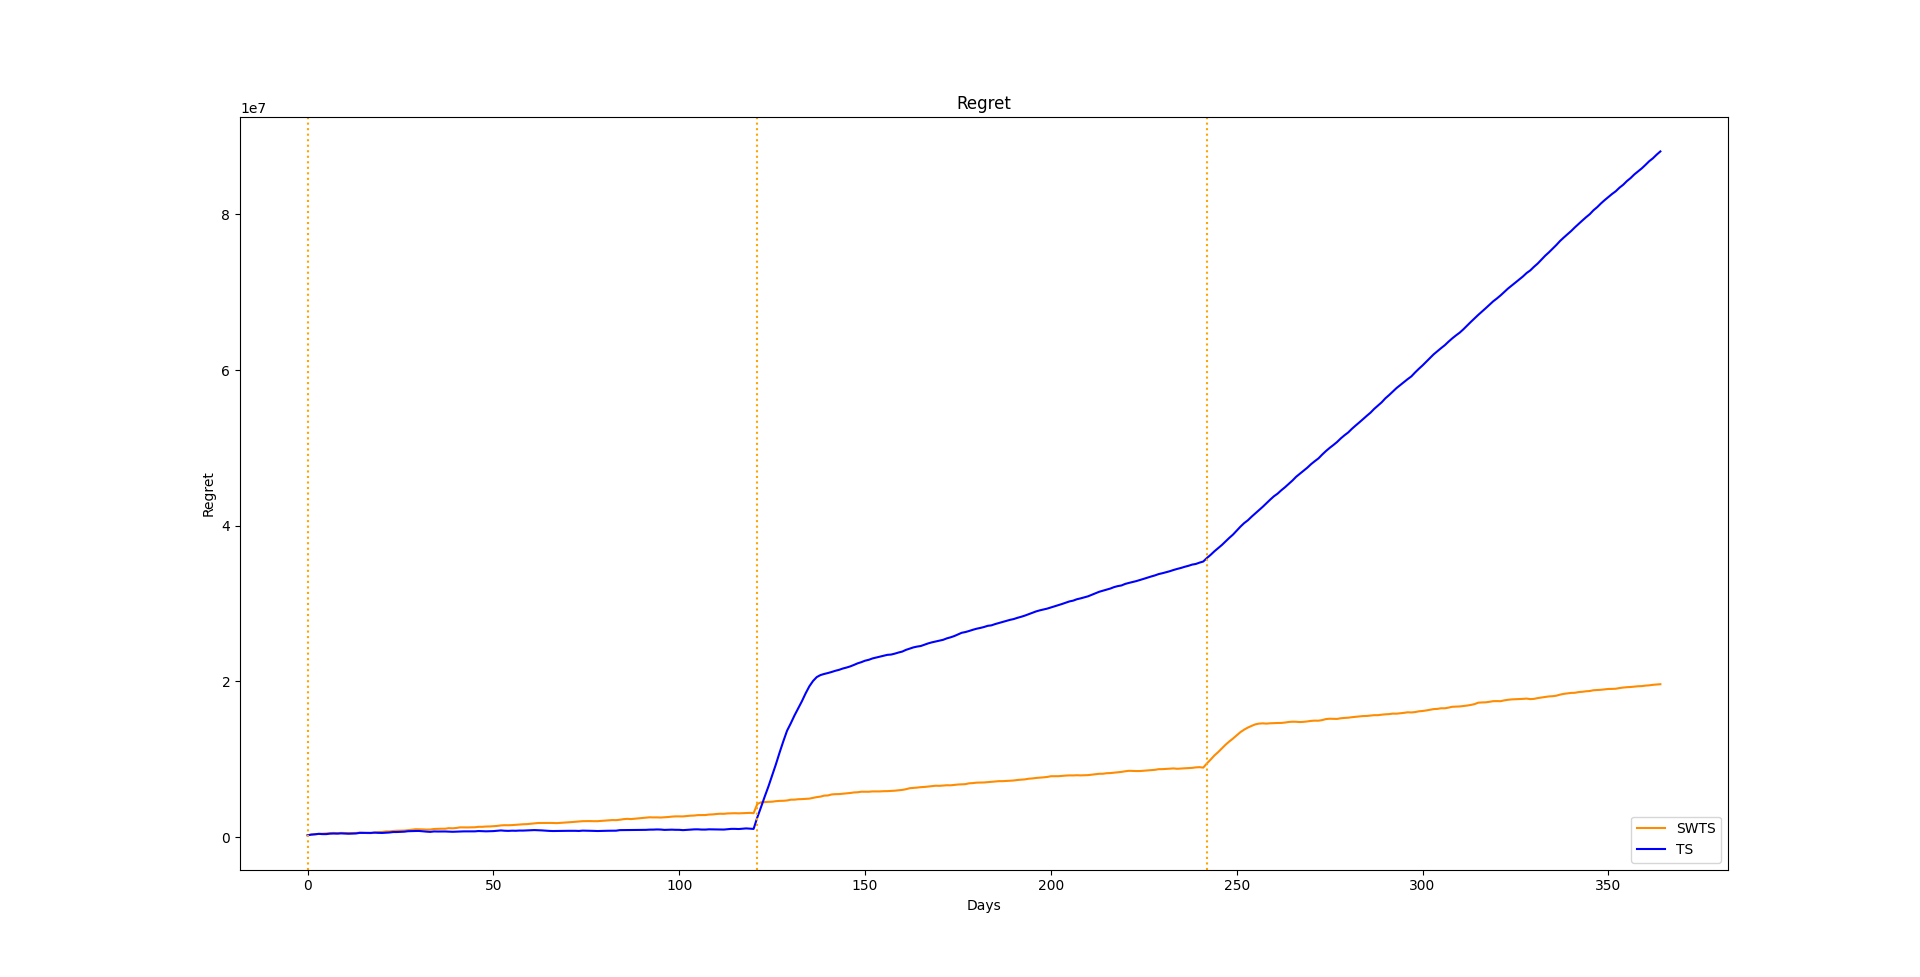
\includegraphics[scale=0.30]{Images/n7}
\end{center}
Days: 365\\
Number of seasons: 3 \\
Season length : $|356/3| = 122 $ days\\
Experiments number: 3 \\
Starting delay of the Promo-Category UCB Matching: 1000 clients\\
SWTS window size : $\sqrt{365 * 1000} * 30$\\
\subsection*{Considerations}
We can observe that in the first season the SW-TS algorithm has an higher regret than the TS algorithm, because the first has a number of samples that is equal to the dimension of the window, instead the second collects all the samples. The SW-TS has a better performance from the second season, due to the sliding-window approach, it stabilizes faster than the TS, and at the end, the cumulative regret for the SW-TS is about 4 times less than the TS.